\section{When is a fine-tune spectrally visible?}
\label{sec:theory}

In an idealized proportional-limit model of a layerwise weight perturbation, we
characterize when a fixed-rank component produces a resolvable spectral outlier.
Fix $W \in \R^{p \times q}$ with $q \le p$, and take
$p,q\to\infty$ with $q/p\to\gamma\in(0,1]$. For finite checkpoints, write the
Base-to-Instruct delta
$\dW = W_{\text{instruct}} - W_{\text{base}}$.
We study the eigenvalues of $C = \tfrac{1}{p}\dW^{\!\top}\dW$, whose nonzero
values are the squared singular values of $\dW$ divided by $p$.

\paragraph{Ideal Gaussian null: iid entries yield a Marchenko--Pastur bulk.}
Our ideal null takes the increment entries to be iid
$\mathcal N(0,\sigma^2)$. The spectrum of $C$ then converges to the
Marchenko--Pastur law on $[\sigma^2(1-\sqrt\gamma)^2,\ \sigma^2(1+\sqrt\gamma)^2]$
\citep{marchenko1967}. The limiting upper edge is
$\lambda_+ = \sigma^2(1+\sqrt\gamma)^2$. Finite null eigenvalues fluctuate around
this edge, so empirical visibility uses the finite-size margin in
Appendix~\ref{app:details}.

\paragraph{The signal: a low-rank spike and its spectral-visibility threshold.}
Model the increment as Gaussian noise plus a deterministic rank-$r$ signal,
$\dW = N + S$, $S = \sum_{i=1}^r \beta_i a_i b_i^{\!\top}$, with the $a_i,b_i$
orthonormal, $r$ fixed, and $\theta_i = \beta_i^2/(p\sigma^2)$ converging to fixed
positive limits. The rectangular additive finite-rank
transition of \citet{benaych2012} shows that, for a single spike under these
assumptions, the leading eigenvalue of $C$ detaches asymptotically if and only if
the spike clears a threshold:
\begin{equation}
\lambda_1(C) \xrightarrow{\text{a.s.}}
\begin{cases}
\sigma^2(1+\theta)\!\left(1+\tfrac{\gamma}{\theta}\right), & \theta > \sqrt\gamma,\\[1.2ex]
\sigma^2(1+\sqrt\gamma)^2, & \theta \le \sqrt\gamma.
\end{cases}
\label{eq:bbp}
\end{equation}
Above threshold, a simple spike's leading right singular vector has overlap
$|\langle \hat v_1, b\rangle|^2 \to (1-\gamma/\theta^2)/(1+\gamma/\theta)$.
It is therefore correlated with, but not generally consistent for, $b$
\citep{benaych2012}. Transposition gives the left singular direction used for
residual interventions at the same dimensionless threshold. Later ablation and
steering experiments separately test the behavioral relevance of empirical
leading subspaces.

The same white-noise formulas occur in the classical Gaussian rank-one spiked
population-covariance model \citep{baik2005,baik2006,paul2007}, historically
associated with the Baik--Ben~Arous--P\'ech\'e transition. Those results use a
multiplicative covariance model; the checkpoint delta here follows the additive
rectangular model above.

\begin{figure}[t]
\centering
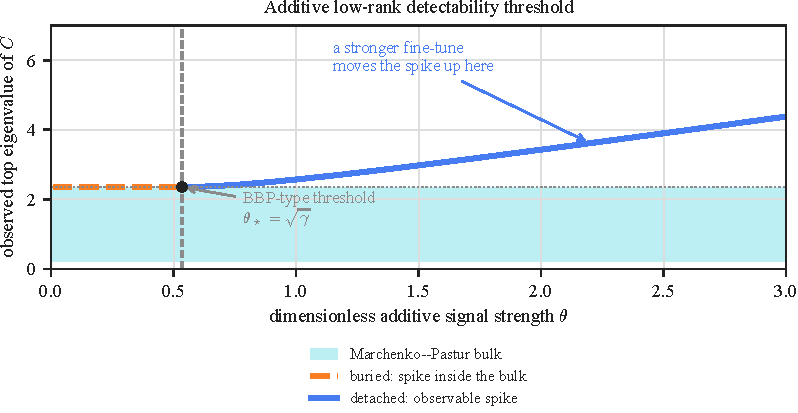
\includegraphics[width=0.62\textwidth]{../results/figures/bbp.pdf}
\caption{The rectangular additive spectral-visibility transition of
Equation~\eqref{eq:bbp} (normalized
$\sigma^2=1$, at the representative aspect ratio $\gamma\approx0.29$ of the feed-forward maps).
Moving right increases planted-signal strength; moving up increases the observed
top eigenvalue. Below $\theta_\star=\sqrt{\gamma}$ the signal remains buried at
the noise edge; above it the detached branch rises and its singular vector acquires
nonzero overlap with the planted direction.}
\label{fig:bbp}
\end{figure}

\paragraph{Rank at fixed energy.}
Writing $\tau = \sum_i \theta_i$ fixes the signal energy
$\|S\|_F^2=p\sigma^2\tau$. An equal-strength rank-$r$ update places $\tau/r$ in
each direction, which clears the threshold
exactly when
\begin{equation}
\frac{\tau}{r} > \sqrt\gamma \quad\Longleftrightarrow\quad r < \rstar := \frac{\tau}{\sqrt\gamma}.
\label{eq:rstar}
\end{equation}
Here $\tau$ is the normalized energy of the latent component $S$, conditional on
the decomposition $\dW=N+S$; it is not directly observed in a checkpoint delta.
For fixed $r$ under the stated spiked model, $\max_i\theta_i\geq\tau/r$ makes
$r<r_\star$ a one-sided guarantee of an outlier. The boundary is exact under
equal strengths; at $r\geq r_\star$, absence of an outlier additionally requires
every $\theta_i\leq\sqrt\gamma$.
Appendix~\ref{app:details} states the known-scale Gaussian Tracy--Widom assumptions
\citep{johnstone2001} and finite-size checks. An equal-strength update below
$r_\star$ therefore yields a spectrally visible signal subspace, whereas one at or above
$r_\star$ remains in the bulk under this model. Interventions separately assess
whether measured behavior is sensitive to the selected empirical subspaces.

\begin{table}[t]
\centering
\caption{Assumption and evidence map. Mathematical claims are conditional on the
listed model; behavioral semantics come from separate experiments.}
\label{tab:assumption-map}
\footnotesize
\begin{tabular}{>{\raggedright\arraybackslash}p{0.19\textwidth}>{\raggedright\arraybackslash}p{0.33\textwidth}>{\raggedright\arraybackslash}p{0.37\textwidth}}
\toprule
statement & status and assumptions & empirical role \\
\midrule
MP upper edge & Established; iid Gaussian entries, $q/p\to\gamma$ & Fitted
reference; Gaussian control at fitted MP bulk scale \\
Detachment and overlap & Established; fixed-rank $S$, isotropic Gaussian $N$,
fixed strength & Synthetic endpoints; interventions are not a quantitative
single-spike test \\
Fixed-energy rank boundary & Corollary; latent signal energy, equal-strength
allocation for the exact boundary & $S$, $\tau$, and $r$ unestimated; matched
scalar summaries show no descriptive separation \\
Behavioral relevance & Empirical; not implied by random-matrix theory & Capture,
matched controls, held-out ranking, and intervention \\
\bottomrule
\end{tabular}
\end{table}
